\appendix

\section{Baseline methods}
\subsection{Geweke test}
The Geweke test \citep{geweke_getting_2004} compares (estimates of) the expectations of hand-picked features (\emph{test functions}) under both the forward and backward joints. 
Specifically, let $g: \mathcal{Y}\times \Theta\to \mathbb{R}$ denote a test function, and let  $S_f=\{(y_i, \theta_i)\}_{i=1}^n$ be samples from the forward joint and $S_b=\{(\tilde{y}_i, \tilde{\theta}_i)\}_{i=1}^n$ be ones from the backward joint.
Then, the z-score 
% $\sqrt{n}(\hat{\bar{g}} - \hat{\tilde{g}})/\sqrt{\hat{\sigma^{2}}+\hat{\tilde{\sigma}}^{2}}$
\begin{equation}
    \frac{\bar{g}(S_f) - \bar{g}(S_b)}{\sqrt{ \frac{\hat{\sigma}^{2}}{N} + \frac{\hat{\tilde{\sigma}}^{2}}{N}}} 
    % \xrightarrow[]{d} \mathcal{N}(0, 1)
    \label{eq:geweke}
\end{equation}
asymptotically follows the standard Gaussian if $\tilde{\pi}(\theta\given y)=\pi(\theta\given y)$, where $\bar{g}(S) = \frac{1}{n}\sum_{(y,\theta) \in S}g(y, \theta)$ and $\hat{\sigma}, \hat{\tilde{\sigma}}$ are estimated variances. 
The width of the window estimator $\hat{\tilde{\sigma}}$ can be set to account for the serial dependence in the backward joint samples.
\subsection{\cite{talts_validating_2018}}
% \cite{talts_validating_2018} take a similar approach under the assumption that the posterior is absolutely continuous.
The authors draw samples using the BC algorithm, then compute univariate rank statistics of a draw from the prior among the thinned, approximately independent posterior samples; if there is no error, the rank statistics should be discretely uniformly distributed. 
The authors suggest examining histograms of the rank statistics to better understand errors rather than conducting a formal test.

\subsection{Rank statistic approach of \cite{gandy_unit_2020}}
The rank test from \cite{gandy_unit_2020} requires reversibility of the MCMC sampler. It draws a sample $\theta_{l}$ from the prior, with the associated index $l$ drawn uniformly from $\{1,\ldots,\tilde{L}\}$. The sampler is then run forward and backward to generate samples $\theta_{1}, \ldots, \theta_{l-1}$ and $\theta_{l+1}, \ldots, \theta_{\tilde{L}} $. Under the null, the rank statistic of $\theta_{l}$ among the other samples should be uniformly distributed; after many repeated simulations, this is verified using a $\chi^{2}$ test.

\section{Experiment details}
\subsection{Experiment 1}
\subsubsection{Effect of sampler mixing speed}
\label{appendix:ex1a}
\begin{figure}[H]
    \centering
    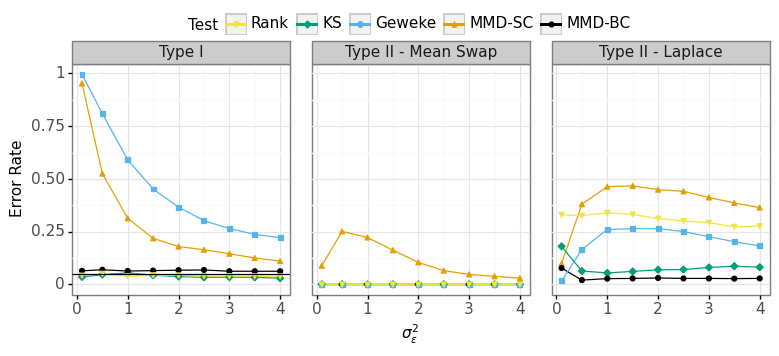
\includegraphics[width=\textwidth]{figures/results_1a.png}
    \caption{Experiment 1 type-I/II error rates against $\sigma_{\epsilon}$, over 1000 trials with a sample size of 250. As $\sigma_{\epsilon}$ increases, autocorrelation in the Gibbs sampler decreases and mixing speed increases. We use the thinning size $t=5$ for the SC simulator, and take $L=500$ burn-in steps for both the SC and BC simulators. For the Rank test, each rank statistic is calculated using a chain of length $\tilde{L}=5$.}
    \label{fig:ex1a}
\end{figure}

\subsubsection{Effect of varying BC simulator burn-in}
\begin{figure}[H]
    \centering
    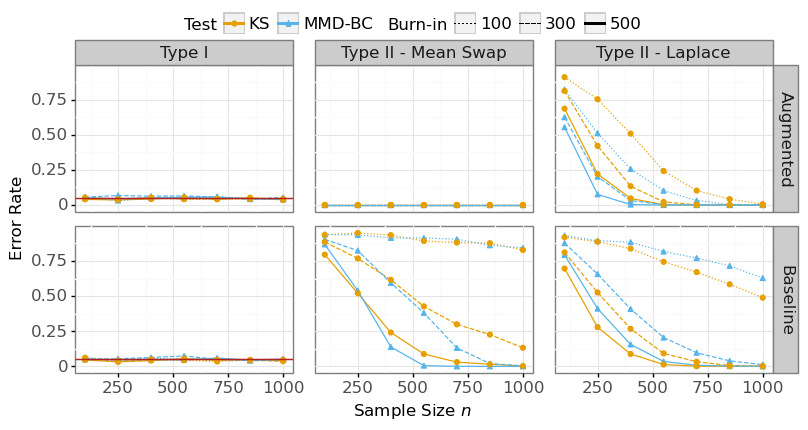
\includegraphics[width=\textwidth]{figures/results_1b.png}
    \caption{Experiment 1 type-I/II error rates over 1000 trials for different burn-in sizes $L$. The top panels use the likelihood- and prior-augmented test functions and the bottom panels use the baseline as discussed in the text. We set $\sigma_{\epsilon}^{2}=0.1$. Type-II error rates fall as the $L$ increases.}
    \label{fig:ex2b}
\end{figure}

\subsection{Experiment 2: Reversible Jump Sampler Implementation}
\label{appendix:ex2}
The prior is defined by
\begin{equation}
  \pi(\theta|\tau, a, b ) = p(\ell|\lambda) p(\mathbf{\gamma}|\ell) p(\sigma^{2} | a, b) \prod_{j} p(\beta_{j} | \tau, \gamma) 
\end{equation}
where
\begin{equation}
  p(\ell|\lambda) = \frac{\exp{(-\lambda)} \lambda^{\ell}}{C\ell!}, \quad \ell \in \{1,\ldots, p\}
\end{equation}
\begin{equation}
  p(\mathbf{\gamma}|\ell) \propto {d\choose \ell}^{-1}
\end{equation}
\begin{equation}
  p(\beta_{j} | \tau, \gamma ) = \begin{cases} (2\tau)^{-1}\exp(-\frac{|\beta_{j}|}{\tau}) & j \in \mathbf{\gamma} \\ \delta(\beta_{j}) & \text{otherwise} \end{cases}
\end{equation}
\begin{equation}
    p(\sigma^{2} | a, b) = \frac{b^{a}}{\Gamma(a)} (\sigma^{2})^{-a-1} \exp{\left(-\frac{b}{\sigma^{2}}\right)}
\end{equation}
$C$ is a normalization constant, $\delta$ is the Dirac delta function, and $\mathbf{\gamma}$ is a vector of the nonzero indices of $\beta$.
The likelihood is given by
\begin{equation}
  p(y | \sigma, \beta, X ) = (2\pi)^{-\frac{n}{2}} \sigma^{-n} \exp{\left(-\frac{\Vert y-X\beta\Vert^{2}_{2}}{2\sigma^{2}}\right)}
\end{equation}
The joint probability is then
\begin{equation}
    \begin{aligned}
         p(y, \theta | X ) \propto &\sigma^{-n} \exp{\left(-\frac{\Vert  y-X\beta\Vert^{2}_{2}}{2\sigma^{2}}\right)} \times \\ 
         & \frac{\exp{(-\lambda)} \lambda^{\ell}}{\ell!} {d\choose \ell}^{-1} \prod_{j\in \mathbf{\gamma}} (2\tau)^{-1}\exp\left(-\frac{|\beta_{j}|}{\tau}\right) \prod_{j' \notin \mathbf{\gamma}} \delta(\beta_{j'}) \frac{b^{a}}{\Gamma(a)} (\sigma^{2})^{-a-1} \exp{\left(-\frac{b}{\sigma^{2}}\right)}
    \end{aligned}
    \label{eq:ex2_joint}
\end{equation}

Each iteration of the reversible-jump MCMC posterior sampler takes two steps in random order. The first is a Gibbs step. By conjugacy,
\begin{equation}
    \sigma^{2} | y, X, \beta \sim \mathcal{IG}\left(a + \frac{n}{2}, b + \frac{\sum_{i=1}^{n}(y_{i}-x_{i}\beta)^{2} }{2}\right)
\end{equation}
where $x_{i}$ denotes row $i$ of $X$.

The second is a reversible jump step. We start by proposing $\ell' \in \{\ell-1, \ell, \ell+1\}$ uniformly at random, disallowing $\ell<1$ and $\ell>p$. Thus, when $\ell \in \{1,p\}$, there are only two valid proposals, not three. Then, depending on the $\ell'$ proposed, we complete the proposal $\tilde{\theta}$ via one of the following
\begin{itemize}
    \item Update: $\ell' = \ell$
    \begin{enumerate}
        \item Choose $j \in \{1, \ldots, \ell\}$ uniformly at random
        \item Propose $\mathbf{\gamma}' = \mathbf{\gamma}, \beta'_{j} = \beta_{j} + \mathcal{N}(0, \epsilon_{\text{update}}), \beta'_{i \neq j} = \beta_{i}$
        \item $P(\tilde{\theta} \rightarrow \theta) = P(\theta \rightarrow \tilde{\theta})=\mathcal{N}(\beta_{j}'; \beta_{j},\epsilon_{\text{update}})=\mathcal{N}(\beta_{j}; \beta_{j}',\epsilon_{\text{update}})$
    \end{enumerate}
\end{itemize}

\begin{itemize}
    \item Birth: $\ell' = \ell+1$
    \begin{enumerate}
        \item Choose $j \in \{\ell+1, \ldots, p\}$ uniformly at random
        \item Propose $\mathbf{\gamma}' = \mathbf{\gamma} \cup j$
        \item Propose $\beta'_{j} = \mathcal{N}(0, \epsilon_{\text{birth}}), \beta'_{i \neq j} = \beta_{i}$
        \item $p(\tilde{\theta} \rightarrow \theta) = \begin{cases}\frac{1}{2}\frac{1}{\ell'} & \ell'=p \\ \frac{1}{3} \frac{1}{\ell'} & 1<\ell<p \end{cases} $
        \item $p(\theta \rightarrow \tilde{\theta}) = \begin{cases}\frac{1}{2}\frac{1}{p-\ell} \mathcal{N}(\beta_{j}'; 0,\epsilon_{\text{birth}}) & \ell=1 \\ \frac{1}{3} \frac{1}{p-\ell} \mathcal{N}(\beta_{j}'; 0,\epsilon_{\text{birth}}) & 1<\ell<p \end{cases} $
    \end{enumerate}
\end{itemize}

\begin{itemize}
    \item Death: $\ell' = \ell-1$
    \begin{enumerate}
        \item Choose $j \in \{1, \ldots, \ell\}$ uniformly at random
        \item Propose $\mathbf{\gamma}' = \mathbf{\gamma} \setminus j$ 
        \item Propose $\beta'_{j} = 0, \beta'_{i \neq j} = \beta_{i}$
        \item $p(\tilde{\theta} \rightarrow \theta) = \begin{cases}\frac{1}{2}\frac{1}{p-\ell'} \mathcal{N}(\beta_{j}; 0,\epsilon_{\text{birth}}) & k'=1 \\ \frac{1}{3} \frac{1}{p-\ell'} \mathcal{N}(\beta_{j}; 0,\epsilon_{\text{birth}}) & 1<\ell'<p \end{cases} $
        \item $p(\theta \rightarrow \tilde{\theta}) = \begin{cases}\frac{1}{2}\frac{1}{\ell} & \ell=p \\ \frac{1}{3} \frac{1}{\ell} & 1<\ell<p \end{cases} $
    \end{enumerate}
\end{itemize}
where $\epsilon_{\text{update}}, \epsilon_{\text{birth}}$ are random walk sizes.

We accept the birth-death proposal $\tilde{\theta}$ with probability 
\begin{equation}
    A(\tilde{\theta}|\theta) = \min{\left(\frac{p(y, \tilde{\theta} |  X, \tau, a, b  )}{p(y, \theta |  X, \tau, a, b  )} \frac{p(\tilde{\theta} \rightarrow \theta)}{p(\theta \rightarrow \tilde{\theta})}, 1\right)} \\
\end{equation}

